\chapter{Scientific Problem}
\label{section:scientificProblem}



\section{Problem definition}
\label{section:problemDefinition}

Before defining the proposed solution, we should first illustrate the problem and analyze it in detail. Based on this in-depth analysis, decisions will be made to choose the best fitted approach from a software development perspective.

Software is a vast term generally used to refer to applications, scripts and programs that run on a device. Yet there are different kinds of software, each one having its own challenges and things to be taken into consideration. Designing and implementing an operating system would involve low-level programming and hardware interaction. On the other hand, this becomes absolutely unnecessary if you're developing an eCommerce software product. Indeed, there are practices and patterns that could be applied to all kinds of software, but many are relevant for only one particular field. That is why, as a first step, we should describe the main characteristics of the application that will be built and identify under what type of software it fits.

First of all, our application would involve persistent data. The data about documents which were added by the users should be stored for several years, allowing users to access it, filter it, generate data reports and make conclusions based on them.

As it will be used by the majority of the employees rather that a single person, the application should ensure that many people can access the data concurrently without causing errors. This is especcialy important for web applications which have thousands or millions of users, but even for a small application like ours, concurrency should be handled in a way that would exclude data consistency and integrity problems.

Then there is the most important part of the application: its business logic. What data should be stored for each document? What input values are considered valid for each field? Who is allowed to view and edit the data? What functionalities should the app provide? The answer to all this questions can only be found by analyzing the requirements of the client and turning them in business rules that would serve as the functional engine of the application.

Last but not least, the application needs to provide a GUI\footnote{Graphical User Interface} that would present the data to the user. The challenge here would be to design the application keeping in mind that usability is as important as functionality. A software system meant to improve the effectiveness of processes in an organization should also offer effectiveness and efficiency in its usage. To bring users satisfaction from interacting with the app, the GUI must provide all the desired features, yet keep things simple and intuitive.

The identified characteristics are also described in \cite{patternsOfEnterpriseApplicationArchitecture} as aspects that define Enterprise Applications as a software type. Enterprise Applications are software solutions that provide business logic to handle processes of an organisation in a way that would improve efficiency and productivity. Some people think of a large system when hearing the term "Enterprise Application". Yet it is important to keep in mind that not all enterprise applications are large and that the value they bring to the organization does not depend on their size. What is also important to understand is that even an application for a small organization, with a few users and relatively simple logic, needs to be build in such a way that will be maintainable and extensible. It could happen that in a couple of years the organization would like to add other proceses to the app, and thus we have to make sure it allows adding new functionality without having to reimplement already existing logic. This can only be achived by taking into account well-known design patterns qualified for our purpose.



\section{Theoretical foundations}
\label{section:theoreticalFoundations}

In this section of the thesis we will analyze the theoretical foundations that will further help us design and build the applciation keeping in mind all the challenges that were previously mentioned.


\subsection{Why a Web distributed system?}
\label{subsection:whyAWebDistributedSystem}

A first and important decision we have to make is whether to develop a desktop application or a web-based one. Indeed, a traditional desktop app doesn't need internet connection in order to be used. However, this seems to be its biggest and only advantage. Web applications, on the other hand, have a wide range of advantages. To start with, a web application runs on a web browser, which means there is no need to install additional software on the the computer from which it will be used. This makes it accessible from a wide range of devices and operating systems. In addition, it gives users freedom to access the app from anywhere, anytime, via any device with an Internet connection, allowing them to solve urgent tasks without a trip to the office. App maintainance is also less complicated - once an update is made on the host server, users can access it without manual updates on their computer. This are the main reasons why building a web application was chosen over a classical desktop one.

% think about the title?
\subsection{Layering architecture}
\label{subsection:layeringArchitecture}

A web application architecture is based on a client-server model, which is a distributed application system that divides tasks between the server - the provider of resources, and the client, which communicates with the server via requests made over the network. As stated in \cite{databaseProgrammingWithJdbcAndJava}, the simplest shape a client-server architecture can take is a two-tier architecture. This originated back in the 90s long before the rise of the popularity of web applications. Back then, it was used in database applications so that the server layer was responsible for data storage and retrieval and the client handled data manipulation and presentation. Nowadays however, applications are much more complex, which calls for the necessity of adding an additional layer responsible for the business logic. This is known as the "three-tier architecture", which consists of three primary layers: Presentation Layer, Application Layer and Database Layer (See Figure \ref{threeTierArchitecture}).

Each of the layers has its own set of responsibilities. The Presentation Layer, in our case a web-browser UI, handles the display of information as well as user requests, such as mouse clicks, keyboard hits and http requests. The Database Layer is primarilly responsible for storing persistent data. The middle-tier, called the Application Layer, is the means of communication between the other two layers and is fully responsible for all the business logic of the application. This includes performing calculations based on user input, validation of the data that comes from the UI, and execution of different business flows depending on requests received from the Presentation Layer.

\begin{figure}[H]
    \centering
    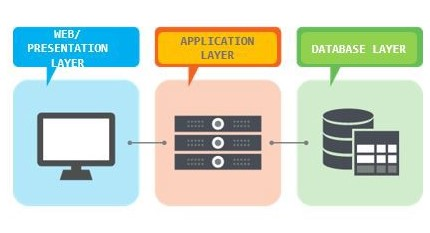
\includegraphics[width=5in]{images/threeTierArchitecture}
    \caption{The three-tier architecture \cite{threeTierArchitecture}}
    \label{threeTierArchitecture}
\end{figure}

The three-tier architecture represents the simplest layering scheme that could be successfully applied to an enterprise application. However, if the application is quite complex, it would indeed need additional mediating layers. This raises the question of how to further split the layers and how the dependencies between layers should be managed. The Software Engineering field has seen quite a few architecture models which serve exactly this purpose.

"The Clean Architecture" seen in Figure \ref{cleanArchitectureImg} is, as described in \cite{cleanArchitecture}, an attemp to integrate and combine several architectures having as end goal the separation of concerns, which results in modular systems composed of fairly independent components.

\begin{figure}[H]
    \centering
    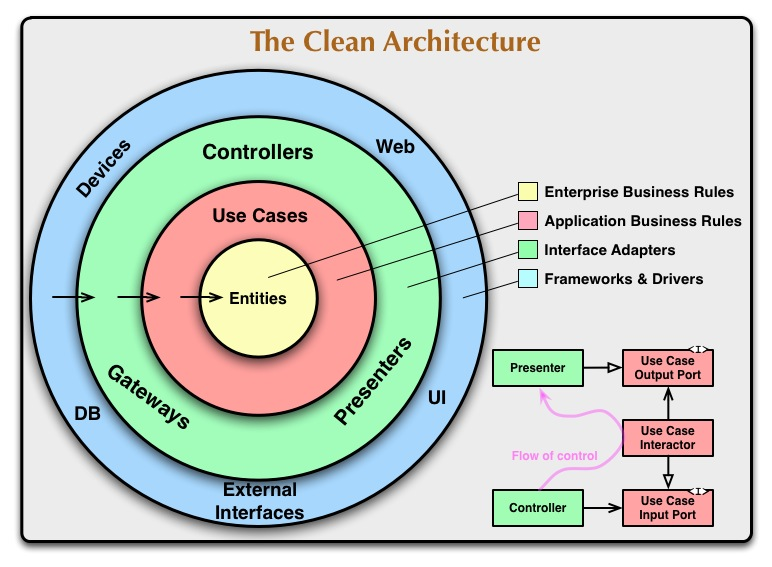
\includegraphics[width=6in]{images/cleanArchitecture}
    \caption{The clean architecture \cite{cleanArchitecture}}
    \label{cleanArchitectureImg}
\end{figure}

The circles in Figure \ref{cleanArchitectureImg} show different components of a software application:

\begin{itemize}
    \item \textbf{Entities} represent the business objects of the application.
    \item \textbf{Use cases} encapsulate the business logic and is not affected by changes to the database or the UI.
    \item \textbf{Interface adapters} act as converters between data formats and handle communication between use cases and entities with the database or the web GUI.
    \item \textbf{Frameworks and drivers} is a layer composed mainly of tools - be it the database or the web framework.
\end{itemize}

Of course, a true clean architecture would imply a low coupling of layers, that would permit the components to remain independent of one another. The business layer should be independent of the database, allowing it to be replaced with a different data source as long as the model objects keep the same structure. At the same time, it should also be independent of the UI. Thus, the UI could change, be redesigned or reimplemented using another framework without even touching the business layer. This separation also contributes to making the business layer highly testable on its own, without involving the actual database or the UI.

To achive this low coupling, an important rule must be kept in mind when defining dependencies between modules and layers. This is described in \cite{cleanArchitecture} as "The Dependency Rule", which states that "Source code dependencies must point only inward". To clarify this, let's look again at Figure \ref{cleanArchitectureImg}. According to the rule, components from an inner circle should not know about components from an outer circle. From a code perspective, this means that any software entity should use only those software entities that were declared in an inner circle. As an example, a controller, which belogs to the Interface Adapters group, cannot use an entity defined in the Web Presentation layer, which belongs to Frameworks and Drivers. Instead, it is the responsiblity of the Web Presentation layer to make a request to the controller, which will then invoke the Application layer and so on.

Building dependencies according to this rule will result in a layered design with a structure that resembles a \textit{directed acyclic graph} (DAG), meaning that it has no cycles. This will ensure that the components are independent of one another, which will make them easier to develop, maintain and extend.


\subsection{Client-server communication: Representational State Transfer}
\label{subsection:rest}

In the previous subsection, we have talked about the separation of client and server so that each one of them could be individually developed and changed without affecting the other part. However, the only way to achive this modularity is to establish a communication standart between the server and the client.

This could be accomplished by using Representational State Transfer (REST), which is an architectural style for providing standards for communication between web systems. It was designed as an alternative to Simple Object Access Protocol (SOAP), which has been, for a long time, the mainly used architectural style for building web services. However, due to its simplicity, lightweightness and scalability, REST has quickly gained popularity and is nowadays the most popular style chosen for web service development.

The decoupling of the client and server is one of the 6 constraints of the REST architectural style. The communication is made via the defined API\footnote{Application Programming Interface} using requests and responses. Clients will send requests using the HTTP protocol and wait for responses. The server will receive those requests and do whatever the client needs, i.e. query the database or perform some other operations. When the REST service will finish processing the reuqest, it will send back a response to the client (See Figure \ref{rest}). It is worth mentioning that the communication is always initiated by the client. The server will never share information about its resources on its own: it will wait and only send responses as reactions to incoming requests.

\begin{figure}[H]
    \centering
    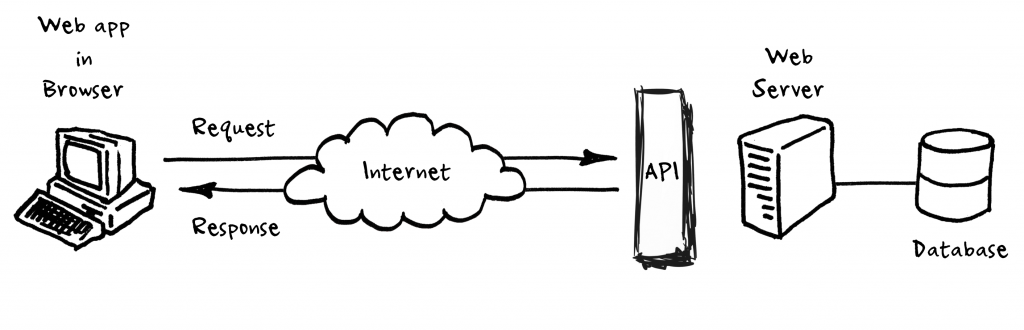
\includegraphics[width=5in]{images/rest}
    \caption{The client-server communication using a REST API \cite{rest}}
    \label{rest}
\end{figure}

What operation will be triggered on the server is determined by the information the client has to provide while making the request:

\begin{itemize}
    \item The \textbf{endpoint}, which is the Uniform Resource Identifier (URI) for the requested resource.
    \item The \textbf{HTTP method} that tells the server which operation needs to be performed on the resource. (See Table \ref{httpVerbs})
\end{itemize}

\begin{table}[H]
    \centering
    \begin{tabular}{|c|l|}
        \hline
        GET    & read a resource             \\ \hline
        POST   & create a new resource       \\ \hline
        PUT    & update an existing resource \\ \hline
        DELETE & delete a resource           \\ \hline
    \end{tabular}
    \caption{The 4 basic HTTP verbs}
    \label{httpVerbs}
\end{table}

Another important REST constraint says that the client-server communication is \textbf{stateless}, meaning that each single client request should contain all the information that the server needs for processing. It does not store a history of the requests and thus cannot use some previous context. Session state management is therefore entirely the client's responsibility. This is one of the main reasons why RESTful web services are so lightweight, scalable and easy to implement.





% - performance (big amount of data)
% - relational vs non-relational db
% - where to store files? (db vs cloud)
% - db stuff (indexing / speeding up things ? highPerformanceMySQL)
% There's usually a lot of data, a moderate system will have over 1GB of data
% organized in tens of millions of records, so much data that managing it is a major part
% of the system. Older systems used indexed file structure such as IBM's VSAM and
% ISAM. Modern systems usually use databases, mostly relational databases. The
% design and feeding of these databases has turned into a sub-profession of its own.


% - architecture/patterns
% - "It is not enough for code to work." Robert C. Martin, Clean Code: A Handbook of Agile Software Craftsmanship


% - security

% - usability (provide all features, yet keep it simple & intuitive)
% - responsiveness vs response time (progress bars page 14)














% just so items from .bib would show up in bibliography
\cite{patternsOfEnterpriseApplicationArchitecture}
\cite{buildingRESTfulWebServicesWithSpring}
\cite{tamingTheStateInReact}
\cite{cleanArchitecture}
\cite{highPerformanceMySQL}
\cite{modernEnterpriseUiDesign}
